% !Mode:: "TeX:UTF-8"

\subsubsection{2.1 研究内容}


\noindent\textbf{2)项目符号和编号}

在多方面多领域得到了广泛的应用:
\begin{itemize}
  \item 军事
  \item 政治
  \item 历史
\end{itemize}
enumerate不同编号\verb+\Alph*,\alph*,\Roman*,\roman*,\arabic*+
系统的分类:
\begin{enumerate}[label=\alph*)]   
  \item 同构系统;
  \item 异构系统。
\end{enumerate}
边距等调整
\begin{enumerate}[leftmargin=2em,itemsep=2pt,topsep=0pt,parsep=0pt,label=\alph*)]  
  \item 考虑只有xxx情形;
  \item 考虑其它情形。
\end{enumerate}

\noindent\textbf{3)公式的插入、对齐}

安装mathtype并根据下图完成配置(图\ref{fig_mathtype1}所示)。
 \begin{figure}[!htb]
  \centering
  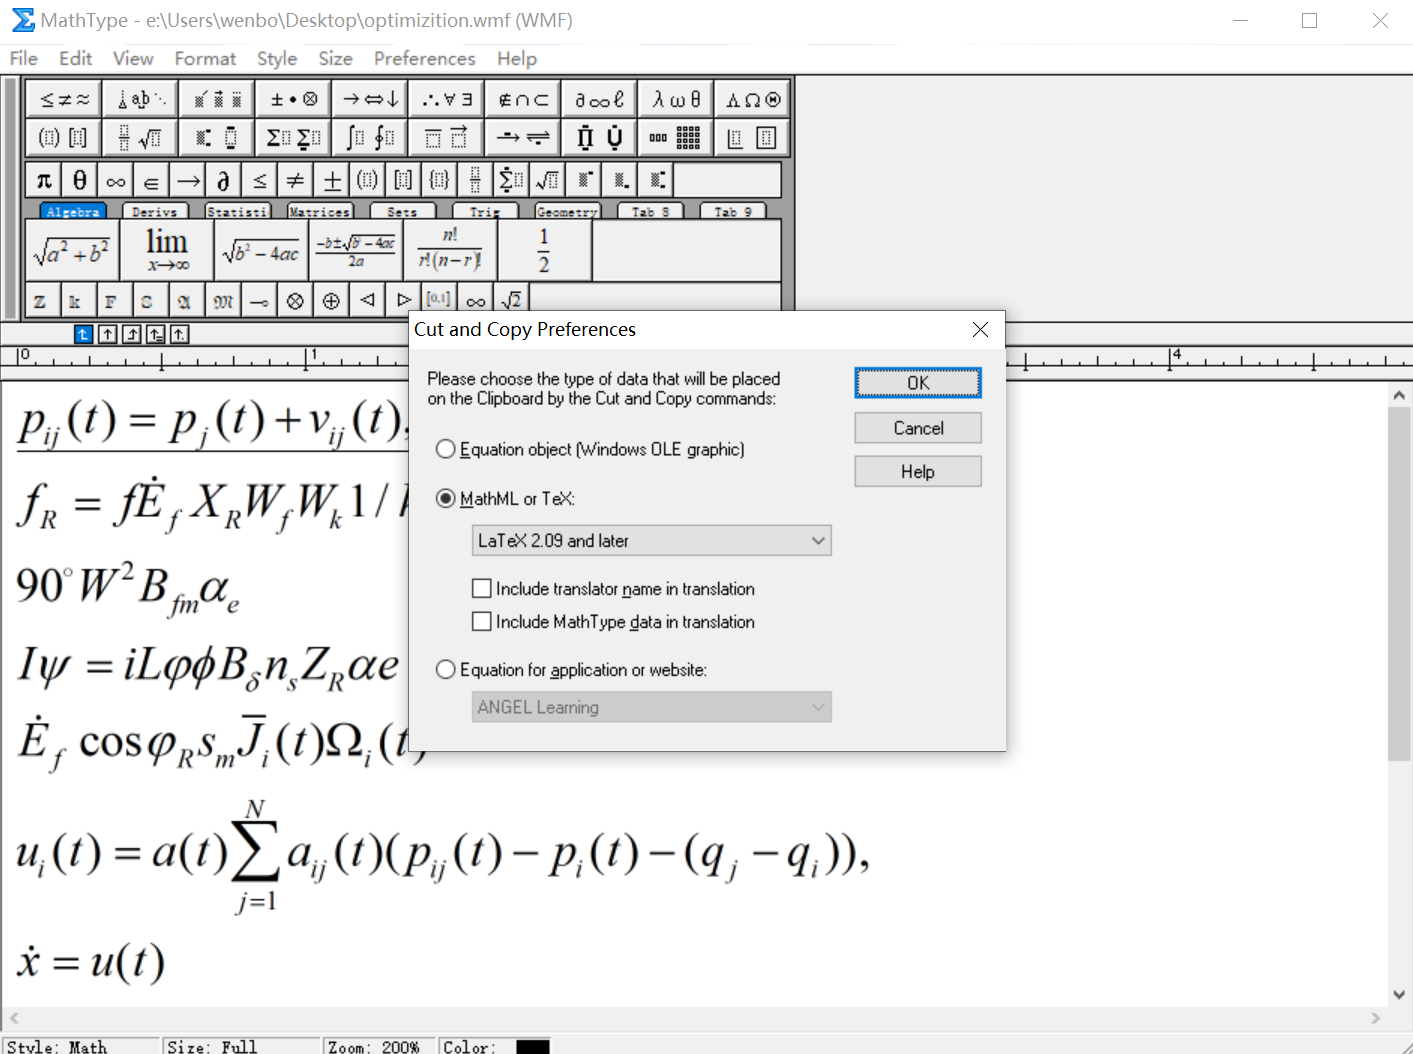
\includegraphics[width=1\textwidth]{mathtype配置}
  \caption{mathtype相关配置.}
  \label{fig_mathtype1}
\end{figure}

在mathtype编辑公式,并从mathtype直接复制到latex,然后进一步修改。

\textcolor{red}{在文字段落中嵌入公式},此时需用到\$符号。下面是详细步骤,首先从mathtype中直接复制过来,不做任何修改,直接编译效果如下
\[{p_{ij}}(t) = {p_j}(t) + {v_{ij}}(t)\]
\textcolor{red}{如果嵌入到一段文字中},需要去掉 \verb|\[|以及\verb|\]|符号,然后用\$包起来,效果是${p_{ij}}(t) = {p_j}(t) + {v_{ij}}(t)$。

如果不嵌入在一段文字中,让公式单独成行,并编号,可以采用下列步骤。
下面公式是直接复制过来,未加任何修改的编译效果。
\[\begin{array}{l}
V(k) \ge a^2+b^2+3\\
 \ge a^2+b^2+2
\end{array}\]

首先需要去掉 \verb|\[|以及\verb|\]|符号,然后用\verb+\begin{equation}以及\end{equation}+来替换。
\begin{equation}\label{system1}
  \begin{array}{l}
V(k) \ge a^2+b^2+3\\
 \ge a^2+b^2+2
\end{array}
\end{equation}

\textcolor{red}{插入不带编号的公式},只需将equation改成\verb+equation*+

但是发现以上的公式并不美观,可以进一步进行对齐完善,\textcolor{red}{仔细对比\eqref{system1}公式代码和\eqref{system2}公式代码的区别},主要先删掉\verb+\begin{array}{l}+以及\verb+\end{array}{l}+,然后要在对齐的地方插入$\&$符号并结合\verb+\begin{split}+指令,完成对齐。

\begin{equation}\label{system2}
\begin{split}
V(k) &\ge a^2+b^2+3\\
 &\ge a^2+b^2+2.
\end{split}
\end{equation}

\textcolor{red}{公式太长的情形,一行放不下的公式,可参考以下进行修改(参考源latex代码进行区分二者的区别)。}举例1如下,下面第一个式子是直接从mathtype复制,第二个式子插入了标签同时进行了对齐(关键看式中的\&符号插入位置和符号$\backslash$$\backslash$的关系)\verb+\hspace{0.3cm}+来表示对齐时空0.3cm


\noindent\textbf{4)列表及算法的插入}

列表插入

\begin{table}[h]
    \caption{工作进度安排}
  \centering
  \setlength{\tabcolsep}{12mm}{
  \begin{tabular}{|c|c|c|}
  \hline
  序号 & 时间                  & 内容      \\ \hline
  1  & 20xx.1.8-20xx.1.12  & xxx     \\ \hline
  2  & 20xx.3.12-20xx.3.18 & xxx   \\ \hline
  \end{tabular}}
  \label{gra_process}
  \end{table}
  
算法设计

  \begin{algorithm}[H]
      \KwIn {西瓜集}
      \KwOut{分类结果}
      初始化\;
      \While{迭代未终止}{
          学习\;
          \eIf{西瓜属性}{
              统计\;
              计算\;
          }{
              下一次迭代\;
          }
      }
      \caption{西瓜集分类算法}
  \end{algorithm}
  


\subsubsection{2.2 研究目标}
本项目的研究目标是

\subsubsection{2.3 拟解决的关键科学问题}


本项目的拟解决



